\documentclass{standalone}

\usepackage{pgfplots}
\usepackage{tikz}
%\usepackage[usenames,dvipsnames]{color}
%\usepackage[dvipsnames]{xcolor}
\usetikzlibrary{shapes, arrows, calc}

\pgfplotsset{compat=1.12}

\definecolor{darkblue}{RGB}{4, 84, 148}
\definecolor{darkred}{RGB}{148, 20, 84}
\definecolor{lightgreen}{RGB}{78, 185, 157}

\tikzstyle{data} = [rectangle, rounded corners, minimum width=0.7cm, minimum height=0.7cm, text centered, draw=black, fill=teal!30]
\tikzstyle{splitdata} = [rectangle split, rectangle split horizontal, rectangle split parts=2, rounded corners, minimum width=0.7cm, minimum height=0.7cm, text centered, draw=black, fill=teal!30]
\tikzstyle{model} = [rectangle, minimum width=0.7cm, minimum height=0.7cm, text centered, draw=black, fill=gray!10]
\tikzstyle{splitmodel} = [rectangle split, rectangle split horizontal, rectangle split parts=2, rounded corners, minimum width=2cm, minimum height=0.4cm, text centered, draw=black, fill=gray!10]
\tikzstyle{prediction} = [ellipse, minimum width=2cm, minimum height=0.5cm, text centered, draw=black, fill=violet!30]
\tikzstyle{concat} = [circle, text centered, draw=black, thick, minimum size=10mm]
\tikzstyle{arrow} = [thick,->,>=stealth]
\tikzstyle{loss} = [ellipse, text centered, draw=black, minimum size=2mm]
\tikzstyle{dot} = [dotted,->,>=stealth]

\begin{document}

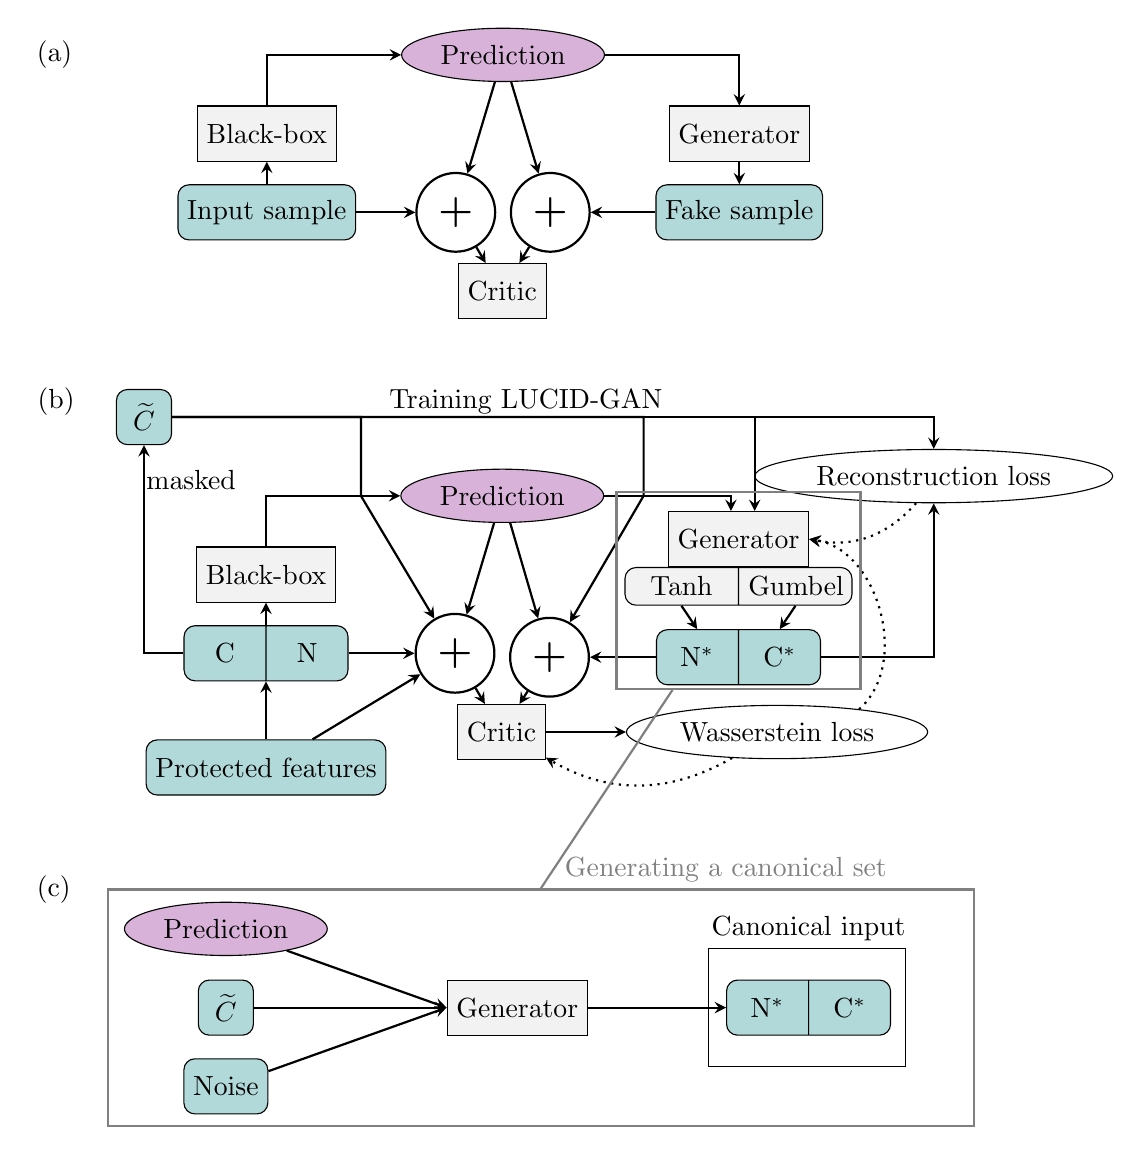
\begin{tikzpicture}

% Figure 1
\node (real) [data] {Input sample};
%\node (fair) [data, below of=real, yshift=-0.45cm] {protected features};
\node (blackbox) [model, above of=real] {Black-box};
\node (pred) [prediction, above of=blackbox, xshift=3cm] {Prediction};
\node (generator) [model, below of=pred, xshift=3cm] {Generator};
\node (fake) [data, below of=generator] {Fake sample};
\node (concatreal) [concat, right of=real, xshift=1.4cm]  {\Large \textbf{+}} ;
\node (concatfake) [concat, left of=fake, xshift=-1.4cm] {\Large \textbf{+}};
\node (critic) [model, below of=concatreal, xshift=0.59cm] {Critic};
%\node (text) [rectangle, right of= critic, minimum width=1cm, minimum height=0.8cm,text centered, xshift=2cm] {fake / real ?};

\draw [arrow] (real) -- (blackbox); %  node[anchor=west] {no}
\draw [arrow] (blackbox) |- (pred);
\draw [arrow] (pred) -| (generator);
\draw [arrow] (generator) -- (fake);
\draw [arrow] (pred) -- (concatreal);
\draw [arrow] (pred) -- (concatfake);
\draw [arrow] (real) -- (concatreal);
%\draw [arrow] (fair) -- (concatreal);
\draw [arrow] (fake) -- (concatfake);
\draw [arrow] (concatreal) -- (critic);
\draw [arrow] (concatfake) -- (critic);
%\draw [arrow] (critic) -- (text);
%\draw [arrow] (fair) -- (real);

% \node [rectangle, above of=pred, xshift=0.3cm, yshift=-0.4cm] {LUCID-GAN overview};

% Figure 2
\node (real_2) [splitdata, below of=critic, text width=0.8cm, xshift=-3cm, yshift=-3.6cm] {\nodepart{one} C \nodepart{two} N};
\node (fair_2) [data, below of=real_2, yshift=-0.45cm] {Protected features};
\node (blackbox_2) [model, above of=real_2] {Black-box};
\node (masked_2) [data, above of=blackbox_2, xshift=-1.55cm, yshift=1cm] {$\widetilde{C}$};
\node (pred_2) [prediction, above of=blackbox_2, xshift=3cm] {Prediction};
\node (generator_2) [model, below of=pred_2, xshift=3cm, yshift=0.45cm] {Generator};
\node (tanhsoft_2) [splitmodel, below of=generator_2, text width=1.2cm, xshift=0cm, yshift=0.4cm] {\nodepart{one} Tanh \nodepart{two} Gumbel};
\node (fake_2) [splitdata, below of=generator_2, text width=0.8cm, yshift=-0.5cm] {\nodepart{one} N$^*$ \nodepart{two} C$^*$};
\node (concatreal_2) [concat, right of=real_2, xshift=1.4cm] {\Large \textbf{+}};
\node (concatfake_2) [concat, left of=fake_2, xshift=-1.4cm] {\Large \textbf{+}};
\node (critic_2) [model, below of=concatreal_2, xshift=0.59cm] {Critic};
\node (loss_2) [loss, right of= critic_2, xshift=2.5cm] {Wasserstein loss};
\node (recon_2) [loss, right of= generator_2, yshift=0.8cm, xshift=1.48cm] {Reconstruction loss};

\draw [arrow] (real_2) -- (blackbox_2);
\draw [arrow] (fair_2) -- (real_2);
\draw [arrow] (blackbox_2) |- (pred_2);
\draw [arrow] (pred_2) -| (generator_2.105);
% \draw [arrow] (generator_2) -- (fake_2);
\draw [arrow] (tanhsoft_2.one south) -- (fake_2.one north);
\draw [arrow] (tanhsoft_2.two south) -- (fake_2.two north);
\draw [arrow] (pred_2) -- (concatreal_2);
\draw [arrow] (pred_2) -- (concatfake_2);
\draw [arrow] (real_2) -- (concatreal_2);
\draw [arrow] (fair_2) -- (concatreal_2);
\draw [arrow] (fake_2) -- (concatfake_2);
\draw [arrow] (concatreal_2) -- (critic_2);
\draw [arrow] (concatfake_2) -- (critic_2);
\draw [arrow] (critic_2) -- (loss_2);

\draw [dot, bend left, thick] (loss_2) edge (critic_2);
\draw [dot, bend right=65, thick] (loss_2) edge (generator_2.east);
\draw [dot, bend left, thick] (recon_2) edge (generator_2.east);

\draw [arrow] (real_2.west) -| node[anchor=west, yshift=2.2cm, xshift=-0.1cm] {masked} (masked_2);

\draw [arrow] (masked_2.east) -| (generator_2.60);
\draw [arrow] (masked_2.east) -| (recon_2);
\draw [arrow] (masked_2.east) -| ($(pred_2.west) - (5mm,0)$) -- (concatreal_2);
\draw [arrow] (masked_2.east) -| ($(pred_2.east) - (-5mm,0)$) -- (concatfake_2);
\draw [arrow] (fake_2.east) -| (recon_2);

\node (rec1) [rectangle, thick, right of=pred_2, xshift=2cm, minimum width=3.1cm, minimum height=2.5cm, yshift=-1.2cm, draw=gray] {};

\node [rectangle, above of=pred_2, xshift=0.3cm, yshift=0.2cm] {Training LUCID-GAN};

% Figure 3
\node (pred_3) [prediction, below of= critic_2, xshift=-3.5cm, yshift=-1.5cm] {Prediction};
\node (mask_3) [data, below of=pred_3] {$\widetilde{C}$};
\node (noise_3) [data, below of=mask_3] {Noise};
\node (generator_3) [model, right of=mask_3, xshift=2.7cm] {Generator};
\node (fake_3) [splitdata, right of=generator_3, xshift=2.7cm, text width=0.8cm] {\nodepart{one} N$^*$ \nodepart{two} C$^*$};

\node (rec2) [rectangle, thick, right of=mask_3, xshift=3cm, minimum width=11cm, minimum height=3cm, yshift=0.0cm, draw=gray] {};
% \node [above of=generator_3, yshift=0.5cm] {};

\node [rectangle, right of=generator_3, draw=black, xshift=2.68cm, minimum width=2.5cm, minimum height=1.5cm, yshift=0.0cm] {};
\node [rectangle, above of=fake_3] {Canonical input};

\node [rectangle, above of=generator_3, text=gray, xshift=2.65cm, yshift=0.75cm] {Generating a canonical set};

\draw [thick, draw=gray] (rec1) -- (rec2.north);

\draw [arrow] (pred_3) -- (generator_3.west);
\draw [arrow] (mask_3) -- (generator_3.west);
\draw [arrow] (noise_3) -- (generator_3.west);

\draw [arrow] (generator_3.east) -- (fake_3.west);

% Annotation
\node [left of=pred, text width=0.8cm, xshift=-4.52cm] {(a)};
\node [below of=critic, text width=0.8cm, xshift=-5.5cm, yshift=-0.4cm] {(b)};
\node [below of=critic_2, text width=0.8cm, xshift=-5.5cm, yshift=-1cm] {(c)};

\end{tikzpicture}

\end{document} 
